\definecolor{preHRcolor}{named}{orange}
\definecolor{postHRcolor}{named}{dinocolor}

\begin{figure}[t]
    \centering
    \begin{subfigure}{0.245\textwidth}
        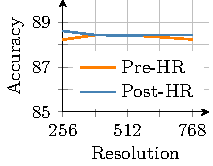
\includegraphics{figures/tikz/post_train_hrft_in1k.pdf}
            \caption{IN1k linear}
        \label{fig:exp:hrft-resolution-in}
    \end{subfigure}%
    \hfill
    \begin{subfigure}{0.245\textwidth}
        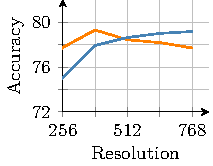
\includegraphics{figures/tikz/post_train_hrft_objectnet.pdf}
        \caption{ObjectNet}
        \label{fig:exp:hrft-resolution-objectnet}
    \end{subfigure}%
    \hfill
    \begin{subfigure}{0.245\textwidth}
        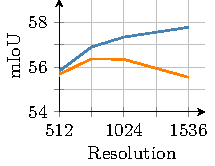
\includegraphics{figures/tikz/post_train_hrft_ade20k.pdf}
        \caption{ADE20k}
        \label{fig:exp:hrft-resolution-ade20k}
    \end{subfigure}%
    \hfill
    \begin{subfigure}{0.245\textwidth}
        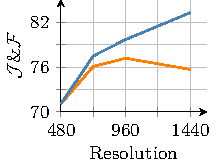
\includegraphics{figures/tikz/post_train_hrft_davis.pdf}
        \caption{DAVIS}
        \label{fig:exp:hrft-resolution-davis}
    \end{subfigure}
    \caption{Effect of high resolution adaptation. 
    Results before (`Pre-HR') and after (`Post-HR') resolution scaling (\cref{sec:algo:hrft}) on (a) linear classification on ImageNet, (b) applied OOD to ObjectNet, (c) linear semantic segmentation on ADE20k, and (d) segmentation tracking on DAVIS at different evaluation resolutions.}
    \label{fig:exp:hrft-resolution}
\end{figure}
